
\section{Data Analysis Method} 
\label{sec:approach}

We are interested in proposing an algorithm with a reduced and prioritized number of validation metrics based on previously acquired validation data (i.e., our dataset). A common method to do this is to identify rules with disjunctive characteristics in the form of a decision tree. The end-goal is to have a decision tree that leads to an outcome that is representative of the overall quality of the comparisons between two signals. In our case, we define such outcome in terms of four categories representative of the quality of the validation: poor, fair, good, excellent. The development of such a decision tree requires a proper classification of the data, which can be done through a clustering process. The following two sections explain the data processing analysis we have put in place to cluster our dataset and obtain two alternative decision trees.

% In machine learning, decision trees are classified as a supervised learning method, and the first step towards designing them requires that the data be labeled according to their attributes. The inherent attribute of our data are the GOF value themselves, but because of the multiplicity of metrics and the lack of clarity about how these relate to each other, we need to add labels to the data that are in accordance with the outcome attributes, i.e., in terms of the predefined validation quality levels. We label the data in our dataset by means of a clustering process. 

% There exist different methods for clustering data \citep[see Chapters 10 and 11 in][]{Han_2011_Book}, among which the \kmeans{} and constrained \kmeans{} clustering methods are the most widely used \citep{Jain_1999_ACMCS}. We note about these methods that the \kmeans{} approach is sensitive to the initial values chosen to be at the center of the clusters---especially in the case of data that are not clearly distinguishable---, whereas the constrained \kmeans{} method uses background knowledge to overcome this limitation. Because of its use of background information, the modified \kmeans{} method is considered as a semi-supervised process.

% Once the data has been properly labeled, one can use a supervised approach to generate the decision tree through a recursive search for the best hypotheses to classify the outcome of the simulation based on a given sub-set of metrics. The following two sections explain the data processing analysis we have put in place to cluster our dataset and obtain the decision tree(s).


\subsection{Clustering}
\label{sec:clustering}

The first step towards obtaining a decision tree is to label the data according to their attributes. The inherent attribute of our data are the GOF values, but because of the multiplicity of metrics and lack of clarity about their relationships, we need to label the data according to the validation categories. We do this by means of a clustering process. 

Clustering is an unsupervised data-mining process used to group data in a multi-dimensional space based on their attributes \citep{Fayyad_1996_IEEE}. According to \citet{Jain_1999_ACMCS}, clustering can be classified in two categories: hierarchical and partitional. Technical details aside, the basic difference is that hierarchical algorithms create nested partitions, whereas partitional algorithms produce singular partitions. 

There is no single clustering process that can be applied to every dataset \citep{Dy_2004_MLR, Jain_1988_Book, Hartigan_1985_JOC}. Consequently, one needs to make choices. We use a partitional, distance-based method known as constrained \kmeans{}. The standard \kmeans{} method is a process for partitioning a $n$-dimensional population into $k$ clusters with a minimum within-cluster attributes variance \citep[e.g.,][]{Macqueen_1967_Proc}. Constrained \kmeans{} extends this method by allowing the use of background information in the form of clustering restrictions.

Given a $k$ number of clusters, where each cluster is identified by its center, the standard process starts by computing the distances of all other data-points to the center of the clusters, and grouping them based on their proximity to the clusters' centers. Once this is done, the center of each cluster is updated based on the average attributes of its data-points, and the process is repeated until the clusters become stable.

\begin{figure}[ht!]
	\centering
	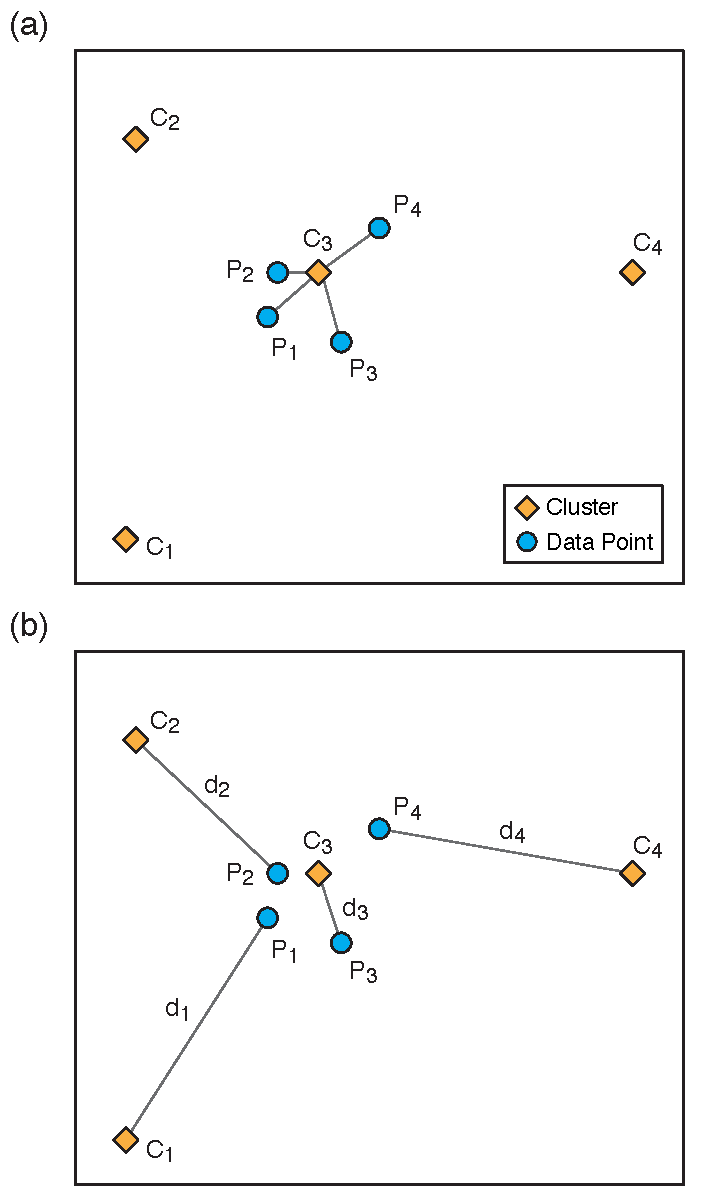
\includegraphics[width=\columnwidth]{figures/pdf/figure-04}
	\caption{Representation of the (a) ordinary, and (b) constrained \kmeans{} approaches for four data-points (P) and four cluster centers (C) in a 2D dataset space, where all the data-points are constrained to be cannot-link points. The color version of this figure is available only in the electronic edition.}
	\label{fig:k-means}
\end{figure}

This process is sensitive to the initial selection of the clusters and their centers. To mitigate this, constrained \kmeans{} introduces two types of constraints: must-link and cannot-link \citep{Wagstaff_2001_Proc}. The must-link constraint specifies instances in which two data-points must be linked, i.e., in the same cluster. The cannot-link constraint specifies instances in which data cannot be in the same cluster. This prevents the process from converging into a local minimum, and defines constrained \kmeans{} as a semi-supervised method. Figure \ref{fig:k-means} illustrates the differences between the standard and constrained \kmeans{} methods for a single clustering iteration on a small two-dimensional dataset.

In our implementation we limit the clustering to four validation categories: poor, fair, good, and excellent. The cluster centers are randomly selected at the start, but we apply constraints by adding 4 artificial stations with cannot-link conditions that are checked at the end of each iteration. These stations are associated with each type of cluster and have GOF scores equal to 3, 5, 7, and 9, across all metrics, thus they are representative of the validation categories. 

In the multi-dimensional space defined by the 11 GOF metrics used here, the distances are obtained using the Euclidean expression:
% 
\begin{equation}
	d(x_i, x_j) = \sqrt{ \sum_{l=1}^{n} \left( x_{i,l} - x_{j,l} \right)^2 } 
\end{equation}
% 
corresponding to the distance $d$ between the data-point $x_i$ and the cluster center $x_j$ in the $n$-dimensional domain, where $x_{i,l}$ is the $l$-th feature of the data-point $x_i$, and $x_{j,l}$ is the $l$-th feature of the cluster center $x_j$. It is, however, unpractical to expect the patterns defining the clusters to be observable across all features. Such high-dimensional issues are well known \citep[see, for instance,][]{Parsons_2004_ACM, Dy_2004_MLR}, and can be tackled using sub-spaces. Therefore, instead of analyzing all $2^{11}$ possible sub-spaces, we focus only on sub-spaces with 2, 3, and 4 dimensions, or features. In total, we analyze 550 sub-spaces, 55 sub-spaces with 2 features, 165 with 3, and 330 with 4.

Unfortunately, not all the sub-spaces will have clearly distinguishable clusters (i.e., some will not satisfy the cannot-link constraints even after a large number of iterations). Such sub-spaces are discarded, and all others are used to label the data. In an ideal case, each station will be labeled 550 times, and the final label is taken as the mode. For example, if after all the sub-spaces are accounted for, a station has labels $\left\{F, F, F, P, F, G, E, F, F\right\}$, where the labels $P$, $F$, $G$, and $E$ correspond to the poor, fair, good, and excellent category clusters, then such as station will be given a final label $F$. Once all the data is properly labeled, we proceed with the decision tree analysis.


% ===========================================================================================
%


% Although we do not expect to see the pattern that resulted from clustering using 11 features in presentation of only two, however, different studies show that the higher dimension reduce the effect of similarity based on distance. \citet{Parsons_2004_ACM} presented an illustrative example to show the effect of dimension in reducing the importance of the distance. Effect of higher dimensions in clustering has been well studied and many different methods are proposed to reduce this effect in the final results. Among them we can name  feature selection before, during, and after clustering, hybrid methods that use combination of methods to select the best subset of feature. \citet{Dy_2004_MLR} addressed two issues involved in developing an automated feature subset selection algorithm for unlabeled data. They illustrated the irrelevant and redundant features and proposed methods for evaluating candidate features using two performance criteria.

% Subspace analysis is another technique to address the challenges with higher dimensional data in clustering process. Subspace clustering is an extension of traditional clustering which looks for different pattern using subset of features.  \citet{Parsons_2004_ACM} provided a list of algorithm for conducting subspace clustering and also some potential applications for them. The most common factor among these algorithm is the process to find a group of best subspaces through optimization process. An n-dimensional dataset has $2^n$ subspaces where it could be very costly and time consuming to evaluate all of them.

% In this study we are interested in using those features who, in general, represent the simulation accuracy in 4 different categories. As a first step we use the constrained \kmeans{} clustering approach for all features, however, because of mentioned reasons the results are not easy to discuss or even evaluate. Although we have four groups of data, the question is which one should be considered as poor, fair, good, or excellent groups. Therefore, we apply a modified method of subspace clustering approach to cluster the stations. As we discussed earlier and presented in figures the constrained \kmeans{} method effectively put the stations in a cluster with considering the fact that our constrain stations should not be in the same cluster. High number of iteration leads the clustering process to follow the clustering concept that we are looking for which is clustering stations as poor, fair, good, and excellent. In our case number of possible subspace is $2^{11}$ where each features have two options wether belong to subspace or not. However, because of preserving the distance based criteria effects we limited the number of features in the subspace to be 2,3, and 4 features. Therefor we have 330,165, and 55 unique subspaces for 4D,3D, and 2D, respectively. We conduct a constrained \kmeans{} clustering analysis for each of these subspaces and repeat the algorithm. In some cases, it is not possible to distinguish all four cannot-link stations in different clusters. In this study we ignore these cases. We only use those combination of features that gives 4 unique clusters for the constraint points (hypothetical stations), therefore, we know for sure that all data within same cluster let's say with metric value 3, should be considered as poor. We also control the clusters to be consistent (we reformat numbers to assign cluster 1 to all group of stations that our first constraint belongs to them and so on). Finally, using 550 unique subspace clustering results, we assign the most frequent class to the station.





% and computes . These distances are then used as a criteria to determine the cluster to which cluster each data-point belongs. 

% ...


% \citet{Macqueen_1967_Proc} describes this method as a process for partitioning a $n$-dimensional population into $k$ sets on the basis of a sample. Its algorithm produces partitions that are reasonably efficient in the sense of within-class variance. It starts with a user defined number of clusters ($k$) and assigns a random mean value to each cluster (or randomly choose $k$ data-points and assigns them as cluster centers). After this, the algorithm computes the distances of all other data-points to the center of the cluster and uses the distance as a criteria to clustering the data points. Because the data resides in a multi-dimensional space (here defined by each metric), there are different ways of computing the distance of each data-point to the cluster's center. We use the Euclidean distance:
% % 
% \begin{equation}
% 	d(x_i, x_j) = \sqrt{ \sum_{k=1}^{n} \left( x_{i,k} - x_{j,k} \right)^2 } 
% 	\, ,
% \end{equation}
% % 
% where $n$ is the number of features and $d$ is the distance of $x_i$ and $x_j$ in $n$-$dimensional$ domain. 




% ===========================================================================================
%
% NEW TEXT PROVIDED BY NAEEM ON JAN 22
% Once the distance is computed, the algorithms labels the data based on the proximity of each point to each cluster, and computes the arithmetic mean value of the data for each cluster, and assigne that value as the updated location of each cluster's center. The algorithm repeats the steps unless the amount of updates among the cluster centers is less than a predefined tolerance value. The major problem with \kmeans{} algorithm is that it is sensitive to the selection of the initial partition and may converge to a local minimum of the criterion function value if the initial partition is not properly chosen. Another problem accompanying the use of \kmeans{} algorithm is the choice of the number of desired output clusters. \citep{Jain_1999_ACMCS}. Clustering is a subjective process. The same set of data items often needs to be partitioned differently for different application. In our application the number of clusters according to the literature is 4 (i.e., poor, fair, good, and excellent.) However, our initial attempts represents that the results are highly sensitive to the initial clusters' center. Therefore, we need to incorporate the experts knowlege in the process. 


% \citet{Wagstaff_2001_Proc}  demonstrated a modification of \kmeans{} clustering algorithm which uses the background information of the domain or dataset. The algorithm adds two types of constraints to the clustering including:
% 	% 
% 	\begin{itemize}
% 	\item{Must-link: constraints specify that two instances have to be in the same cluster.}
% 	\item{Cannot-link: constraints specify that two instance must not be placed in the same cluster.}
% 	\end{itemize} 
% 	% 
% The algorithm is described in detail in \citet{Wagstaff_2001_Proc}, however, in simple words, in the ordinary \kmeans{} process before assigning data to the closes cluster, it controls the must-link and cannot-link conditions. Therefore, in this case, the closest cluster's center is not necessarily the final cluster of the data.


% In a hypothetical assumption, if we have a pair of data and synthetic with GOF score of 3 for all metrics we could consider the overall simulation GOF as poor. This is also correct for 5,7, and 9 that we can assigne them fair, good, and excellent class, respectively. Therefore, we add 4 hypothetical stations into the dataset with GOF score of 3,5,7,and 9 for all metrics and we put them in cannot-link constraint. This assumption that originated from the experts knowledge, provides enough information to the algorithm to converge to the same final clusters and cluster centers after a reasonable amount of iteration. 

% Fig.~\ref{fig:con_kmeans} presents the difference between ordinary and constrained k-means clustering approach using 4 points and 4 cluster centers. Fig.~\ref{fig:con_kmeans}.a presents the \kmeans{} without constrained. According to the definition and the explanation in this section, the closest cluster center for each points will get the points. 	Fig.~\ref{fig:con_kmeans}.b represents the constrained \kmeans{} approach, where, the closest cluster center is not necessarily the final cluster. The data points can not be in the same cluster, in result,  we assign them to different clusters in this case to satisfy the Cannot-link criteria. The best configuration happens when we minimize the distance between cluster centers and points.

% ===========================================================================================
% 
% OLD STUFF DONE BY RICARDO FOR THE INTRO OF THIS SECTION
% 
% In machine learning, decision trees are classified as a supervised learning method, and the first step towards designing them requires that the data be labeled according to their attributes. The inherent attribute of our data are the GOF value themselves, but because of the multiplicity of metrics and the lack of clarity about how these relate to each other, we need to add labels to the data that are in accordance with the outcome attributes, i.e., in terms of the predefined validation quality levels. We label the data in our dataset by means of a clustering process. 

% There exist different methods for clustering data \citep[see Chapters 10 and 11 in][]{Han_2011_Book}, among which the \kmeans{} and constrained \kmeans{} clustering methods are the most widely used \citep{Jain_1999_ACMCS}. We note about these methods that the \kmeans{} approach is sensitive to the initial values chosen to be at the center of the clusters---especially in the case of data that are not clearly distinguishable---, whereas the constrained \kmeans{} method uses background knowledge to overcome this limitation. Because of its use of background information, the modified \kmeans{} method is considered as a semi-supervised process.





% ===========================================================================================
%
% SECOND ATTEMPT THAT WAS RECALLED BY NAEEM

% Once the distance is computed, the algorithms labels the data based on the proximity of each point to each cluster, computes the mean value of the data for each cluster, and updates the location of each cluster's center. \textcolor{red}{(How do we compute ``mean value'' and how do we recompute the ``center''? All what follows after this in the original text is too descriptive, and not specific enough. We need to go to the point and this is going in long description circles.)} 

% {\color{gray}
% 	The algorithm repeats the steps unless the amount of updates among the cluster centers is less than a tolerance value.  \kmeans{} clustering has been applied in different applications, however, there is no clustering technique that is universally applicable in uncovering the variety of structures present in multidimensional datasets. Therefore, clustering is a subjective process. The same set of data items often needs to be partitioned differently for different application. In result, it is essential for the user of a clustering algorithm to not only have a thorough understanding of the particular technique being utilized, but also to know the details of the data gathering process and to have some domain expertise; the more information the user has about the data at hand, the more likely the algorithm would be able to succeed in assessing its true class structure. Domain concept can play several roles in the clustering process, and a variety of choices are available to the practitioner \citep{Jain_1999_ACMCS}. 

% 	The major problem with \kmeans{} algorithm is that it is sensitive to the selection of the initial partition and may converge to a local minimum of the criterion function value if the initial partition is not properly chosen. Another problem accompanying the use of \kmeans{} algorithm is the choice of the number of desired output clusters. Several variant of the \kmeans{} algorithm have been reported in the literature. Some of them attempt to select a good initial partition so that the algorithm is more likely to find the global minimum value, another variation is to permit splitting and merging of the resulting clusters \citep{Jain_1999_ACMCS}. 

% 	In our application the number of clusters is not a problem and there is a consensus among researchers in the number of clusters (i.e., poor, fair, good, excellent), however, our initial attempts represent that the results are highly sensitive to the initial clusters' center. 

% 	Every clustering algorithm uses some type of knowledge either implicitly or explicitly. In this study the background knowledge is a series of hypothetical stations. We assume that there are four stations with score of 3, 5, 7, and 9 for all of their metrics. Based on the score limits in section.~\ref{validation_metrics} we know these stations belong to poor, fair, good, and excellent classes, respectively. These background knowledge could help the clustering processing to be in right direction regarding the fact that increasing dimension of data could increase noise in clustering and cause difficulty to better partitioning. \citet{Wagstaff_2001_Proc}  demonstrated a modification of \kmeans{} clustering algorithm which uses the background information of the domain or dataset. The algorithm adds two types of constraints to the clustering including:
% 	% 
% 	\begin{itemize}
% 	\item{Must-link: constraints specify that two instances have to be in the same cluster.}
% 	\item{Cannot-link: constraints specify that two instance must not be placed in the same cluster.}
% 	\end{itemize} 
% 	% 
% 	The algorithm is described in detail in \citet{Wagstaff_2001_Proc}, however, in simple words, in the ordinary \kmeans{} process before assigning data to the closes cluster, it controls the must-link and cannot-link conditions. Therefore, in this case, the closest cluster's center is not necessarily the final cluster of the data. Fig.~\ref{fig:con_kmeans} presents the difference between ordinary and constrained k-means clustering approach using 4 points and 4 cluster centers. Fig.~\ref{fig:con_kmeans}.a presents the \kmeans{} without constrained. According to the definition and the explanation in this section, the closest cluster center for each points will get the points.
	
% 	Fig.~\ref{fig:con_kmeans}.b represents the constrained \kmeans{} approach, where, the closest cluster center is not necessarily the final cluster. The data points can not be in the same cluster, in result,  we assign them to different clusters in this case to satisfy the Cannot-link criteria. The best configuration happens when we minimize the distance between cluster centers and points. Using this method at each step the algorithm redistribute the 4 hypothetical stations to satisfy the cannot-link constraint. The visual inspection of the figures also confirms the accuracy of the method. Doing this, in the next iteration this data manipulation leads the cluster center in a direction to have the hypothetical station in the cluster and loose those data that is in far other side direction of the hypothetical station. Therefore, the cluster tend to have all data that similar to the hypothetical station. \\
% 	The end product of the clustering process is groups of data. Analysis of these groups, individually, gives the idea about the clusters in terms of within class variation. In these analysis we mainly study the behavior of different features in each cluster and isolate only the most descriptive features to be used in the supervised classifier that assumes a given number of classes in the data set. In the next section we provide a basics of decision tree algorithm. 

% }

% In other words, the points cannot be in the same cluster. In the constrained \kmeans{} approach we redistribute the points such that the $\sum{d}$ becomes minimum.

% ===========================================================================================
%
% OLD NAEEM VERSION
% 
% Clustering is an unsupervised approach for grouping of data based on measure of similarity and it is considered as an exploratory activity as a part of data mining process \citep{Fayyad_1996_IEEE}. In each valid cluster, patterns are more similar in each other than they are to pattern belonging to a different cluster. Many clustering algorithms are developed for different application, however, study the difference of them is beyond the scope of this paper. In general, at the top level,  \citet{Jain_1999} distinguished the clustering approach into Hierarchical and Partitional approaches. Aside from differences in application and technical details in implementation, hierarchical methods produce nested series of partitions, while partitional methods produce only one. In this study we are interested in using partitional, distance based clustering algorithm, which is also known as \kmeans{} algorithm.  \citet{Macqueen_1967_Proc}  described a process for partitioning an $n$-$dimensional$ population into $k$ sets on the basis of a sample. The process appears to give partitions which are reasonably efficient in the sense of within-class variance. For numerical values, \kmeans{} algorithm starts with a user defined number of clusters (k) and assign a random mean value for each cluster (or randomly choose k data and assign them as cluster centers.) Then it computes the distance of data and cluster centers. A variety of distance measures are in use in different studies, however, we use the Euclidean distance through 

% \begin{equation}
% d(x_i,x_j)=\sqrt{\Sigma_{k=1}^{n}(x_{i,k} - x_{j,k})^2},
% \end{equation}

% where $n$ is the number of features and $d$ is the distance of $x_i$ and $x_j$ in $n$-$dimensional$ domain. After computing the distance of the points from each clusters' mean (center), the algorithm continues with labeling the data after the closest cluster. At the next iteration, it computes the mean value of data for each cluster and updates the clusters' centers. The algorithm repeats the steps unless the amount of updates among the cluster centers is less than a tolerance value.  \kmeans{} clustering has been applied in different applications, however, there is no clustering technique that is universally applicable in uncovering the variety of structures present in multidimensional datasets. Therefore, clustering is a subjective process. The same set of data items often needs to be partitioned differently for different application. In result, it is essential for the user of a clustering algorithm to not only have a thorough understanding of the particular technique being utilized, but also to know the details of the data gathering process and to have some domain expertise; the more information the user has about the data at hand, the more likely the algorithm would be able to succeed in assessing its true class structure. Domain concept can play several roles in the clustering process, and a variety of choices are available to the practitioner \citep{Jain_1999}. 

% The major problem with \kmeans{} algorithm is that it is sensitive to the selection of the initial partition and may converge to a local minimum of the criterion function value if the initial partition is not properly chosen. Another problem accompanying the use of \kmeans{} algorithm is the choice of the number of desired output clusters. Several variant of the \kmeans{} algorithm have been reported in the literature. Some of them attempt to select a good initial partition so that the algorithm is more likely to find the global minimum value, another variation is to permit splitting and merging of the resulting clusters \citep{Jain_1999}. 

% In our application the number of clusters is not a problem and there is a consensus among researchers in the number of clusters (i.e., poor, fair, good, excellent), however, our initial attempts represent that the results are highly sensitive to the initial clusters' center. 

% Every clustering algorithm uses some type of knowledge either implicitly or explicitly. In this study the background knowledge is a series of hypothetical stations. We assume that there are four stations with score of 3, 5, 7, and 9 for all of their metrics. Based on the score limits in section.~\ref{validation_metrics} we know these stations belong to poor, fair, good, and excellent classes, respectively. These background knowledge could help the clustering processing to be in right direction regarding the fact that increasing dimension of data could increase noise in clustering and cause difficulty to better partitioning. \citet{Wagstaff_2001_Proc}  demonstrated a modification of \kmeans{} clustering algorithm which uses the background information of the domain or dataset. The algorithm adds two types of constraints to the clustering including:\\
% \begin{itemize}
% \item{Must-link: constraints specify that two instances have to be in the same cluster.}
% \item{Cannot-link: constraints specify that two instance must not be placed in the same cluster.}
% \end{itemize} 
% The algorithm is described in detail in \citet{Wagstaff_2001_Proc}, however, in simple words, in the ordinary \kmeans{} process before assigning data to the closes cluster, it controls the must-link and cannot-link conditions. Therefore, in this case, the closest cluster's center is not necessarily the final cluster of the data. Fig.~\ref{fig:con_kmeans} presents the difference between ordinary and constrained k-means clustering approach using 4 points and 4 cluster centers. Fig.~\ref{fig:con_kmeans}.a presents the \kmeans{} without constrained. According to the definition and the explanation in this section, the closest cluster center for each points will get the points.
% Fig.~\ref{fig:con_kmeans}.b represents the constrained \kmeans{} approach, where, the closest cluster center is not necessarily the final cluster. The data points can not be in the same cluster, in result,  we assign them to different clusters in this case to satisfy the Cannot-link criteria. The best configuration happens when we minimize the distance between cluster centers and points. Using this method at each step the algorithm redistribute the 4 hypothetical stations to satisfy the cannot-link constraint. The visual inspection of the figures also confirms the accuracy of the method. Doing this, in the next iteration this data manipulation leads the cluster center in a direction to have the hypothetical station in the cluster and loose those data that is in far other side direction of the hypothetical station. Therefore, the cluster tend to have all data that similar to the hypothetical station. \\
% The end product of the clustering process is groups of data. Analysis of these groups, individually, gives the idea about the clusters in terms of within class variation. In these analysis we mainly study the behavior of different features in each cluster and isolate only the most descriptive features to be used in the supervised classifier that assumes a given number of classes in the data set. In the next section we provide a basics of decision tree algorithm. 


% \begin{figure}
%     \centering
%     \includegraphics
%       %  [width=\columnwidth]
%         [width=200px]
%         {figures/pdf/Figure_4.pdf}
%     \caption{ Representation of ordinary (a) and constrained (b) \kmeans{} approach. There are four data points (p) and four cluster centers (c) as a sample of $2$-$Dimensional$ dataset. All points are defined as cannot-link constraints. In other words, the points cannot be in the same cluster. In the constrained \kmeans{} approach we redistribute the points such that the $\sum{d}$ becomes minimum.}
%     \label{fig:con_kmeans}
% \end{figure}



% 
\subsection{Decision Trees}
\label{sec:decision-tree}

Building decision trees is a supervised learning process used to approximate a target function as a sequence of disjunctive conditions designed to measure the effectiveness of a set of attributes to classify data and predict outcomes. The theory behind decision trees is well established \citep[e.g.,][]{Quinlan_1986_ML, Mitchell_1997_Book}. 
\myrevision{A decision tree can be used to classify a case by starting at the root of the tree and moving through it until the leaf is encountered. Each tree is a structure including a root, decision nodes and leaf nodes. Decision nodes specifies some test to carried out on attributes and leaf nodes indicate the final class \citep{Quinlan_1993_Book}.} Decision trees are, however, non-unique. They depend on the dataset, the user parameters, and the algorithm employed to build them \citep{Murthy_1998_DMKD}. Therefore, before describing our choice of the decision tree algorithm and parameters, we revise three aspects about the dataset: data classes, attributes equivalence, and dataset balance.

First, regarding data classes we refer to whether the classes of data are properly distinguishable or not, and to whether the data attributes contribute to those classes or not. In our case, data classes are handled by means of the clustering and labeling process. As we described in the previous section, at the end of the clustering process, all the data-points (or samples) in our dataset get labeled with one out of four outcome classes (or clusters) defined in terms of the validation categories (poor, fair, good, excellent).

Second, attributes equivalence refers to whether the data attributes are comparable with each other on equivalent terms or not. There are cases, either because of the method or because of the data, that the data attributes need to be standardized. In artificial neural networks, for instance, the data needs to be normalized on a $[-1,1]$ or $[0,1]$ scale. Normalization is also necessary when data attributes come in different unit scales or value ranges \citep[e.g.,][]{Wu_2010_JH}. In our case, this is not necessary because (a) all the data attributes---defined by the 11 GOF metrics---are on the same dimensionless numerical scale (varying from 0 to 10), and (b) because the algorithm we use is not susceptible to the attributes scale.

Last, there is the issue of balance. A balanced dataset is one that has about the same number of samples per class. Algorithms used for building decision trees tend to perform better with balanced datasets \citep[e.g.,][]{Branco_2016_ACMCS, Weiss_2003_JAIR}. Imbalanced datasets, on the other hand, are those with a significant disparity in the number of samples in each class. Imbalanced datasets can be improved by a resampling process. There are two basic resampling approaches: undersampling and oversampling \citep{Branco_2016_ACMCS}. Undersampling discards data from the subsets with larger number of samples. Oversampling replicates data until reaching appropriate number of samples. Both processes are done by randomly picking data to either be discarded or replicated. In our case, as we will see later, we apply oversampling to one of our dataset classes. This process has consequences, mainly that it increases the likelihood of overfitting. \myremove{A matter we discuss later.} \myrevision{Overfitting happens when the prediction algorithm predicts the final results too closely or exactly to the training data, however, it provides non-accurate results for unseen or test data.}

Upon completing the clustering and resampling processes, the next step is to subdivide the dataset in two, a training dataset (with 70 percent of the samples picked randomly), and a testing dataset (with the remaining 30 percent). We first use the training dataset to build a large suite of potential decision trees, and then use the testing dataset to evaluate and pick the best possible decision tree(s) among them. There are several algorithms for building decision trees \citep[e.g., ID3, C4.5, C5.0, CART; see][]{Quinlan_1986_ML, Quinlan_1993_Book, Quinlan_1996_JAIR, Breiman_1984_Book}. \myrevision{C5.0 is considered as the developed version of ID3 and C4.5, where it does not have any limitations in handling missing data, numerical attributes, and developing boosted models. Internal algorithm of CART is different than other methods, however, discussing technical details of these algorithms are beyond the scope of this study.} Here we use the C5.0 implementation \citep{Kuhn_2017_Manual}, which is an extension of the C4.5 algorithm developed by \citet{Quinlan_1993_Book, Quinlan_1996_JAIR}.

In essence, given a dataset, the process of building the tree consists of recursively identifying the attributes in the training data that are most likely to predict an outcome. The process is recursive because new branches and decision nodes are created based on the remaining data at every branch and level, until the tree reaches a certain depth or when other conditions are met. The effectiveness of an attribute $A$ in classifying any subset $S$ from the training data is measured through the information gain $G$ as
% 
\begin{equation}
	\label{eq:gain}
	G(S,A) = E(S) - \sum_{v \, \in \, A[a]} \frac{ \left| S_v \right| }{ \left| S \right| } E \left( S_v \right)
	\, ,
\end{equation} 
% 
where $A[a]$ is the set of all possible values of attribute $A$, $S_v$ is the subset of $S$ for which attribute $A$ has value $v$, and $E(\cdot)$ is the entropy function given by
% 
\begin{equation}
	E(S) = \sum_{i=1}^{c} \Big( -p_i \log_2 \left(p_i\right) \Big)
	\, ,
\end{equation}
% 
where $p_i$ is the proportion of $S$ belonging to class $i$, and $c$ are the different values that a given target attribute can take.

Entropy measures the homogeneity of a set of data. The higher the entropy, the more even the distribution of the data across classes. Conversely, an extremely low value of entropy would mean most of the data falls within a particular class. With this in mind, the information gain $G$ of an attribute $A$ for the dataset $S$, or $G(S,A)$ in equation (\ref{eq:gain}), is the expected reduction in entropy caused by partitioning the dataset according to attribute $A$ \citep{Mitchell_1997_Book}. For selection of a threshold for a \myrevision{numerical} continuous attribute refer to \citet{Quinlan_1996_JAIR}.

In the particular case of the C5.0 algorithm the result of this process depends on several parameters, logical and numerical. We set the options to do feature selection \myrevision{or winnowing. Therefore, the algorithm choose to use the most important attributes and ignore others. We also activate the evaluation of possible advanced splits of data. Sometimes data is very close to the splitting threshold where assigning a hard threshold may incorrectly change the classification, whereas, that small difference could happen because of numerical errors or error in measurement. Therefore, advanced split can define a soft threshold to consider different probabilities in assigning data to different classes. A decision tree can grow so deep to finally classify all training data correctly. However, the tree will be very complex and will suffer from overfitting. In other words it will have very poor functionality for test data. Therefore, decision tree algorithms (here C5.0) first grow the tree up to the most complex tree then based on user defined factors start to prune the grown tree.The pruning process helps to reduce the complexity of the tree and also increase it's generalizability. Consequently the pruned tree's leaf nodes will have training data which belongs to more than one class which the final class will be the mode of that leaf node. In this study we use two parameters to control the pruning process including confidence or certainty factor (CF) and the smallest number of samples that must be put in at least two of the splits ($S_{\min}$, also known as \textit{minCases}). C5.0 algorithm uses error-based pruning method (see \citet{Quinlan_1993_Book} for more details). The objective is to minimize the observed error rate. Therefore, error estimates for leaf nodes and subtrees are computed assuming that they were used to classify a set of unseen cases with a predicted error rate which is computed based on CF and binomial distribution of number of misclassified events (E) and all training data at that leaf (N). Decreasing CF and increasing $S_{\min}$ cause more heavy pruning process \citep[see][]{Kuhn_2017_Manual}.} \myremove{and evaluate possible advanced splits of data, but do not use the boosted models option \citep[see][]{Kuhn_2017_Manual}; and use the confidence factor (CF) and the smallest number of samples that must be placed in at least two of the splits ($S_{\min}$, also known as \textit{minCases}) to fine tune the prediction models.} In particular, we build a suite of trees for varying values of CF and $S_{\min}$.



Each tree resulting from this process has different qualities. We are interested in selecting a tree that is highly effective, but with a low level of complexity. In other words, we seek a tree with a good ratio of accuracy for predicting the classification outcome of the data, while using a reduced number of attributes (GOF metrics) in only a few number of steps (as given by a small number of decision nodes or a tree with shallow depth). The number of metrics, the number of nodes, and the depth of a tree are directly seen from the topology of the tree, and are often proportional (shallow trees tend to use less nodes, and thus less metrics). In general, smaller trees are preferable because they are easy to understand and often more accurate predictors \citep{Quinlan_1996_JAIR}.

The effectiveness of the tree, on the other hand, needs to be measured. To that end we use the factor $F_{\beta}$ proposed by \citet{Rijsbergen_1979_Book} as
% 
\begin{equation}
	\label{eq:f}
	F_{\beta} = \frac{ (1 + \beta^2) P R}{\beta^2 P + R}
	\, ,
\end{equation}
% 
where $P$ and $R$ are the precision and recall factors, respectively, and $\beta$ is a weighting factor between the two. $P$ measures the fraction of data samples that are correctly classified within a category, whereas $R$ measures the fraction of the data classified within that category regardless of whether it was correctly classified or not. Mathematically, they are defined as
% 
\begin{equation}
	P = \frac{ \mathrm{TP} }{ \mathrm{TP} + \mathrm{FP} } 
	\quad \mathrm{and} \quad
	R = \frac{ \mathrm{TP} }{ \mathrm{TP} + \mathrm{FN} }
	\, .
\end{equation}
% 
Here, TP, FP, and FN are the number of samples in the testing dataset considered to be true-positives, false-positives, and false-negatives, respectively. These values are typically ordered in what is known as a confusion matrix. For the simplest case of two categories, a confusion matrix takes the form
% 
\begin{equation}
\nonumber
\begin{array}{rr@{}rl}
	&					&	\multicolumn{2}{c}{\mathrm{Prediction}}		\\
	&					&	\mathrm{Positive}	&	\mathrm{Negative}	\\[0.75ex]
	\mathrm{Actual~Value}		
	&	\begin{array}{r}
			\mathrm{Positive} \\[1ex]
			\mathrm{Negative} 
		\end{array}
	&	\left[~
		\begin{array}{c}
			\mathrm{TP} \\[1ex]
			\mathrm{FP} 
		\end{array}\right.
	&
		\left.
		\begin{array}{cc}
			~\mathrm{FN} \\[1ex]
			~\mathrm{TN} \\[1ex]
		\end{array}~\right]
\end{array}
\end{equation}
% 
where TN is the number of true-negative samples.

We compute $F_{\beta}$ in equation (\ref{eq:f}) using $\beta = 1$ to give equal weight to $P$ and $R$ \citep{McCarthy_1995_Proc}. This is done for all the trees obtained using all possible combinations of CF and $S_{\min}$ values. Then, we select the tree with the highest level of effectiveness as \myremove{measure} \myrevision{measured} by $F_1$, commensurate to such tree having a low complexity, i.e., a reduced number of metrics and a shallow depth, which is precisely the goal set at the start. Note that $F_1$ is obtained based on the testing dataset as opposed to the training dataset. The results as applied to our dataset are presented next.


% =========================================================================================================================
% 
% NAEEM NEW SUGGESTION
% 
% Prioritized, reduced number of validation metrics requires developing a decision-making algorithm. A common method to do this is to identify rules with disjunctive characteristics in the form of a decision tree. Decision tree is considered as a supervised learning method. Therefore, we need to know the overall GOF of each observation in the dataset. Or in other words if we consider the simulation process for that specific station and component as poor, fair, good, or excellent process.  Therefore, the first step in such an approach requires that the data be labeled according to their attributes. The inherent attribute of our data is the GOF value, but need to label the data in terms of the outcome attribute. Generating labels for data is mainly possible through a clustering process. There exist different methods for clustering data (see Chapter 10 and 11 of Han 2011). The k-means and constrained k -means clustering methods are among the most widely used Ease of implementation, simplicity, efficiency, and empirical success are the main reasons for its popularity (Jain 2010). We note about these methods that the k –means approach is sensitive to the initial values chosen as the center of the clusters—especially in the case of data that are not clearly distinguishable—, whereas the constrained k –means method uses background knowledge to overcome this limitation. Because of its used of background information, the modified k -means method is considered as a semi-supervised process. Once the data has been properly labeled, one can use a supervised approach to generate the decision tree that can serve as a prediction model for the outcome. In essence, the process of designing the decision tree is a search for the best hypothesis to classify the outcome of the simulation, i.e., the similarity between synthetic and recorded seismograms, based on a given sub-set of metrics. The following two sections explain the data processing analysis we have put in place to achieve this.

% =========================================================================================================================
% 
% RICARDO FIRST PASS

% In order to study the relationships that exist between the different validation metrics and offer a prioritized, reduced number of metrics that can help predict validation results, we need to identify and classify patterns in the dataset. A common method to do this is to identify rules with disjunctive characteristics in the form of a decision tree. Among the available approaches used to design such a tree there are machine learning methods that use supervised and unsupervised learning. The first step in such an approach requires that the data be labeled according to their attributes. The inherent attribute of our data is the GOF value, but need to label the data in terms of the outcome attribute. Following common practice, in our case, we want to label the dataset values as poor, fair, good, or excellent.

% Generating labels for data in an automated way is possible through a clustering process. There exist different methods for clustering data (see \textcolor{red}{a reference about clustering}). The \kmeans{} and modified \kmeans{} clustering methods are among the most widely used (\textcolor{red}{a reference to back up this statement}). We note about these methods that the \kmeans{} approach is sensitive to the initial values chosen at the center of the clusters---especially in the case of data that are not clearly distinguishable---, whereas the modified \kmeans{} method uses background knowledge to overcome this limitation. Because of its used of background information, the modified \kmeans{} method is considered as a semi-supervised process.

% Once the data has been properly labeled, one can use a supervised approach to generate the decision tree that can serve as a prediction model for the outcome. In essence, the process of designing the decision tree is a search for the best hypothesis to classify the outcome of the simulation, i.e., the similarity between synthetic and recorded seismograms, based on a given sub-set of metrics. The following two sections explain the data processing analysis we have put in place to achieve this.

% 
\subsection{Clustering}
\label{sec:clustering}

The first step towards obtaining a decision tree is to label the data according to their attributes. The inherent attribute of our data are the GOF values, but because of the multiplicity of metrics and lack of clarity about their relationships, we need to label the data according to the validation categories. We do this by means of a clustering process. 

Clustering is an unsupervised data-mining process used to group data in a multi-dimensional space based on their attributes \citep{Fayyad_1996_IEEE}. According to \citet{Jain_1999_ACMCS}, clustering can be classified in two categories: hierarchical and partitional. Technical details aside, the basic difference is that hierarchical algorithms create nested partitions, whereas partitional algorithms produce singular partitions. 

There is no single clustering process that can be applied to every dataset \citep{Dy_2004_MLR, Jain_1988_Book, Hartigan_1985_JOC}. Consequently, one needs to make choices. We use a partitional, distance-based method known as constrained \kmeans{}. The standard \kmeans{} method is a process for partitioning a $n$-dimensional population into $k$ clusters with a minimum within-cluster attributes variance \citep[e.g.,][]{Macqueen_1967_Proc}. Constrained \kmeans{} extends this method by allowing the use of background information in the form of clustering restrictions.

Given a $k$ number of clusters, where each cluster is identified by its center, the standard process starts by computing the distances of all other data-points to the center of the clusters, and grouping them based on their proximity to the clusters' centers. Once this is done, the center of each cluster is updated based on the average attributes of its data-points, and the process is repeated until the clusters become stable.

\begin{figure}[ht!]
	\centering
	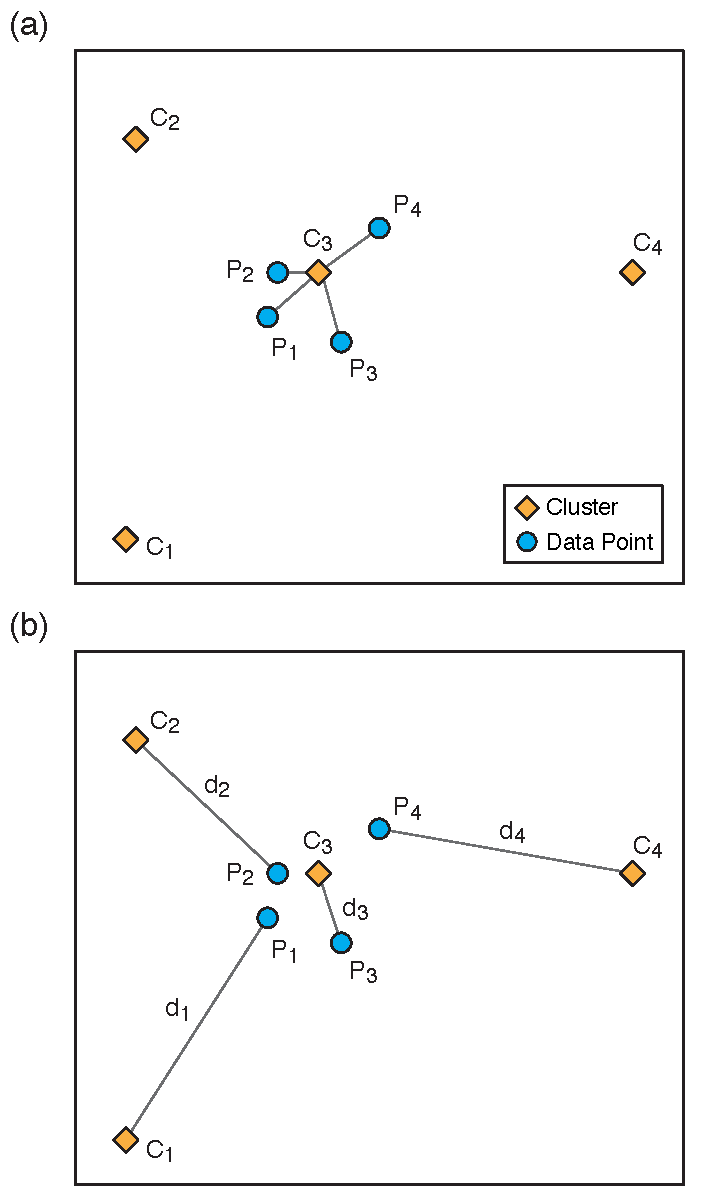
\includegraphics[width=\columnwidth]{figures/pdf/figure-04}
	\caption{Representation of the (a) ordinary, and (b) constrained \kmeans{} approaches for four data-points (P) and four cluster centers (C) in a 2D dataset space, where all the data-points are constrained to be cannot-link points. The color version of this figure is available only in the electronic edition.}
	\label{fig:k-means}
\end{figure}

This process is sensitive to the initial selection of the clusters and their centers. To mitigate this, constrained \kmeans{} introduces two types of constraints: must-link and cannot-link \citep{Wagstaff_2001_Proc}. The must-link constraint specifies instances in which two data-points must be linked, i.e., in the same cluster. The cannot-link constraint specifies instances in which data cannot be in the same cluster. This prevents the process from converging into a local minimum, and defines constrained \kmeans{} as a semi-supervised method. Figure \ref{fig:k-means} illustrates the differences between the standard and constrained \kmeans{} methods for a single clustering iteration on a small two-dimensional dataset.

In our implementation we limit the clustering to four validation categories: poor, fair, good, and excellent. The cluster centers are randomly selected at the start, but we apply constraints by adding 4 artificial stations with cannot-link conditions that are checked at the end of each iteration. These stations are associated with each type of cluster and have GOF scores equal to 3, 5, 7, and 9, across all metrics, thus they are representative of the validation categories. 

In the multi-dimensional space defined by the 11 GOF metrics used here, the distances are obtained using the Euclidean expression:
% 
\begin{equation}
	d(x_i, x_j) = \sqrt{ \sum_{l=1}^{n} \left( x_{i,l} - x_{j,l} \right)^2 } 
\end{equation}
% 
corresponding to the distance $d$ between the data-point $x_i$ and the cluster center $x_j$ in the $n$-dimensional domain, where $x_{i,l}$ is the $l$-th feature of the data-point $x_i$, and $x_{j,l}$ is the $l$-th feature of the cluster center $x_j$. It is, however, unpractical to expect the patterns defining the clusters to be observable across all features. Such high-dimensional issues are well known \citep[see, for instance,][]{Parsons_2004_ACM, Dy_2004_MLR}, and can be tackled using sub-spaces. Therefore, instead of analyzing all $2^{11}$ possible sub-spaces, we focus only on sub-spaces with 2, 3, and 4 dimensions, or features. In total, we analyze 550 sub-spaces, 55 sub-spaces with 2 features, 165 with 3, and 330 with 4.

Unfortunately, not all the sub-spaces will have clearly distinguishable clusters (i.e., some will not satisfy the cannot-link constraints even after a large number of iterations). Such sub-spaces are discarded, and all others are used to label the data. In an ideal case, each station will be labeled 550 times, and the final label is taken as the mode. For example, if after all the sub-spaces are accounted for, a station has labels $\left\{F, F, F, P, F, G, E, F, F\right\}$, where the labels $P$, $F$, $G$, and $E$ correspond to the poor, fair, good, and excellent category clusters, then such as station will be given a final label $F$. Once all the data is properly labeled, we proceed with the decision tree analysis.


% ===========================================================================================
%


% Although we do not expect to see the pattern that resulted from clustering using 11 features in presentation of only two, however, different studies show that the higher dimension reduce the effect of similarity based on distance. \citet{Parsons_2004_ACM} presented an illustrative example to show the effect of dimension in reducing the importance of the distance. Effect of higher dimensions in clustering has been well studied and many different methods are proposed to reduce this effect in the final results. Among them we can name  feature selection before, during, and after clustering, hybrid methods that use combination of methods to select the best subset of feature. \citet{Dy_2004_MLR} addressed two issues involved in developing an automated feature subset selection algorithm for unlabeled data. They illustrated the irrelevant and redundant features and proposed methods for evaluating candidate features using two performance criteria.

% Subspace analysis is another technique to address the challenges with higher dimensional data in clustering process. Subspace clustering is an extension of traditional clustering which looks for different pattern using subset of features.  \citet{Parsons_2004_ACM} provided a list of algorithm for conducting subspace clustering and also some potential applications for them. The most common factor among these algorithm is the process to find a group of best subspaces through optimization process. An n-dimensional dataset has $2^n$ subspaces where it could be very costly and time consuming to evaluate all of them.

% In this study we are interested in using those features who, in general, represent the simulation accuracy in 4 different categories. As a first step we use the constrained \kmeans{} clustering approach for all features, however, because of mentioned reasons the results are not easy to discuss or even evaluate. Although we have four groups of data, the question is which one should be considered as poor, fair, good, or excellent groups. Therefore, we apply a modified method of subspace clustering approach to cluster the stations. As we discussed earlier and presented in figures the constrained \kmeans{} method effectively put the stations in a cluster with considering the fact that our constrain stations should not be in the same cluster. High number of iteration leads the clustering process to follow the clustering concept that we are looking for which is clustering stations as poor, fair, good, and excellent. In our case number of possible subspace is $2^{11}$ where each features have two options wether belong to subspace or not. However, because of preserving the distance based criteria effects we limited the number of features in the subspace to be 2,3, and 4 features. Therefor we have 330,165, and 55 unique subspaces for 4D,3D, and 2D, respectively. We conduct a constrained \kmeans{} clustering analysis for each of these subspaces and repeat the algorithm. In some cases, it is not possible to distinguish all four cannot-link stations in different clusters. In this study we ignore these cases. We only use those combination of features that gives 4 unique clusters for the constraint points (hypothetical stations), therefore, we know for sure that all data within same cluster let's say with metric value 3, should be considered as poor. We also control the clusters to be consistent (we reformat numbers to assign cluster 1 to all group of stations that our first constraint belongs to them and so on). Finally, using 550 unique subspace clustering results, we assign the most frequent class to the station.





% and computes . These distances are then used as a criteria to determine the cluster to which cluster each data-point belongs. 

% ...


% \citet{Macqueen_1967_Proc} describes this method as a process for partitioning a $n$-dimensional population into $k$ sets on the basis of a sample. Its algorithm produces partitions that are reasonably efficient in the sense of within-class variance. It starts with a user defined number of clusters ($k$) and assigns a random mean value to each cluster (or randomly choose $k$ data-points and assigns them as cluster centers). After this, the algorithm computes the distances of all other data-points to the center of the cluster and uses the distance as a criteria to clustering the data points. Because the data resides in a multi-dimensional space (here defined by each metric), there are different ways of computing the distance of each data-point to the cluster's center. We use the Euclidean distance:
% % 
% \begin{equation}
% 	d(x_i, x_j) = \sqrt{ \sum_{k=1}^{n} \left( x_{i,k} - x_{j,k} \right)^2 } 
% 	\, ,
% \end{equation}
% % 
% where $n$ is the number of features and $d$ is the distance of $x_i$ and $x_j$ in $n$-$dimensional$ domain. 




% ===========================================================================================
%
% NEW TEXT PROVIDED BY NAEEM ON JAN 22
% Once the distance is computed, the algorithms labels the data based on the proximity of each point to each cluster, and computes the arithmetic mean value of the data for each cluster, and assigne that value as the updated location of each cluster's center. The algorithm repeats the steps unless the amount of updates among the cluster centers is less than a predefined tolerance value. The major problem with \kmeans{} algorithm is that it is sensitive to the selection of the initial partition and may converge to a local minimum of the criterion function value if the initial partition is not properly chosen. Another problem accompanying the use of \kmeans{} algorithm is the choice of the number of desired output clusters. \citep{Jain_1999_ACMCS}. Clustering is a subjective process. The same set of data items often needs to be partitioned differently for different application. In our application the number of clusters according to the literature is 4 (i.e., poor, fair, good, and excellent.) However, our initial attempts represents that the results are highly sensitive to the initial clusters' center. Therefore, we need to incorporate the experts knowlege in the process. 


% \citet{Wagstaff_2001_Proc}  demonstrated a modification of \kmeans{} clustering algorithm which uses the background information of the domain or dataset. The algorithm adds two types of constraints to the clustering including:
% 	% 
% 	\begin{itemize}
% 	\item{Must-link: constraints specify that two instances have to be in the same cluster.}
% 	\item{Cannot-link: constraints specify that two instance must not be placed in the same cluster.}
% 	\end{itemize} 
% 	% 
% The algorithm is described in detail in \citet{Wagstaff_2001_Proc}, however, in simple words, in the ordinary \kmeans{} process before assigning data to the closes cluster, it controls the must-link and cannot-link conditions. Therefore, in this case, the closest cluster's center is not necessarily the final cluster of the data.


% In a hypothetical assumption, if we have a pair of data and synthetic with GOF score of 3 for all metrics we could consider the overall simulation GOF as poor. This is also correct for 5,7, and 9 that we can assigne them fair, good, and excellent class, respectively. Therefore, we add 4 hypothetical stations into the dataset with GOF score of 3,5,7,and 9 for all metrics and we put them in cannot-link constraint. This assumption that originated from the experts knowledge, provides enough information to the algorithm to converge to the same final clusters and cluster centers after a reasonable amount of iteration. 

% Fig.~\ref{fig:con_kmeans} presents the difference between ordinary and constrained k-means clustering approach using 4 points and 4 cluster centers. Fig.~\ref{fig:con_kmeans}.a presents the \kmeans{} without constrained. According to the definition and the explanation in this section, the closest cluster center for each points will get the points. 	Fig.~\ref{fig:con_kmeans}.b represents the constrained \kmeans{} approach, where, the closest cluster center is not necessarily the final cluster. The data points can not be in the same cluster, in result,  we assign them to different clusters in this case to satisfy the Cannot-link criteria. The best configuration happens when we minimize the distance between cluster centers and points.

% ===========================================================================================
% 
% OLD STUFF DONE BY RICARDO FOR THE INTRO OF THIS SECTION
% 
% In machine learning, decision trees are classified as a supervised learning method, and the first step towards designing them requires that the data be labeled according to their attributes. The inherent attribute of our data are the GOF value themselves, but because of the multiplicity of metrics and the lack of clarity about how these relate to each other, we need to add labels to the data that are in accordance with the outcome attributes, i.e., in terms of the predefined validation quality levels. We label the data in our dataset by means of a clustering process. 

% There exist different methods for clustering data \citep[see Chapters 10 and 11 in][]{Han_2011_Book}, among which the \kmeans{} and constrained \kmeans{} clustering methods are the most widely used \citep{Jain_1999_ACMCS}. We note about these methods that the \kmeans{} approach is sensitive to the initial values chosen to be at the center of the clusters---especially in the case of data that are not clearly distinguishable---, whereas the constrained \kmeans{} method uses background knowledge to overcome this limitation. Because of its use of background information, the modified \kmeans{} method is considered as a semi-supervised process.





% ===========================================================================================
%
% SECOND ATTEMPT THAT WAS RECALLED BY NAEEM

% Once the distance is computed, the algorithms labels the data based on the proximity of each point to each cluster, computes the mean value of the data for each cluster, and updates the location of each cluster's center. \textcolor{red}{(How do we compute ``mean value'' and how do we recompute the ``center''? All what follows after this in the original text is too descriptive, and not specific enough. We need to go to the point and this is going in long description circles.)} 

% {\color{gray}
% 	The algorithm repeats the steps unless the amount of updates among the cluster centers is less than a tolerance value.  \kmeans{} clustering has been applied in different applications, however, there is no clustering technique that is universally applicable in uncovering the variety of structures present in multidimensional datasets. Therefore, clustering is a subjective process. The same set of data items often needs to be partitioned differently for different application. In result, it is essential for the user of a clustering algorithm to not only have a thorough understanding of the particular technique being utilized, but also to know the details of the data gathering process and to have some domain expertise; the more information the user has about the data at hand, the more likely the algorithm would be able to succeed in assessing its true class structure. Domain concept can play several roles in the clustering process, and a variety of choices are available to the practitioner \citep{Jain_1999_ACMCS}. 

% 	The major problem with \kmeans{} algorithm is that it is sensitive to the selection of the initial partition and may converge to a local minimum of the criterion function value if the initial partition is not properly chosen. Another problem accompanying the use of \kmeans{} algorithm is the choice of the number of desired output clusters. Several variant of the \kmeans{} algorithm have been reported in the literature. Some of them attempt to select a good initial partition so that the algorithm is more likely to find the global minimum value, another variation is to permit splitting and merging of the resulting clusters \citep{Jain_1999_ACMCS}. 

% 	In our application the number of clusters is not a problem and there is a consensus among researchers in the number of clusters (i.e., poor, fair, good, excellent), however, our initial attempts represent that the results are highly sensitive to the initial clusters' center. 

% 	Every clustering algorithm uses some type of knowledge either implicitly or explicitly. In this study the background knowledge is a series of hypothetical stations. We assume that there are four stations with score of 3, 5, 7, and 9 for all of their metrics. Based on the score limits in section.~\ref{validation_metrics} we know these stations belong to poor, fair, good, and excellent classes, respectively. These background knowledge could help the clustering processing to be in right direction regarding the fact that increasing dimension of data could increase noise in clustering and cause difficulty to better partitioning. \citet{Wagstaff_2001_Proc}  demonstrated a modification of \kmeans{} clustering algorithm which uses the background information of the domain or dataset. The algorithm adds two types of constraints to the clustering including:
% 	% 
% 	\begin{itemize}
% 	\item{Must-link: constraints specify that two instances have to be in the same cluster.}
% 	\item{Cannot-link: constraints specify that two instance must not be placed in the same cluster.}
% 	\end{itemize} 
% 	% 
% 	The algorithm is described in detail in \citet{Wagstaff_2001_Proc}, however, in simple words, in the ordinary \kmeans{} process before assigning data to the closes cluster, it controls the must-link and cannot-link conditions. Therefore, in this case, the closest cluster's center is not necessarily the final cluster of the data. Fig.~\ref{fig:con_kmeans} presents the difference between ordinary and constrained k-means clustering approach using 4 points and 4 cluster centers. Fig.~\ref{fig:con_kmeans}.a presents the \kmeans{} without constrained. According to the definition and the explanation in this section, the closest cluster center for each points will get the points.
	
% 	Fig.~\ref{fig:con_kmeans}.b represents the constrained \kmeans{} approach, where, the closest cluster center is not necessarily the final cluster. The data points can not be in the same cluster, in result,  we assign them to different clusters in this case to satisfy the Cannot-link criteria. The best configuration happens when we minimize the distance between cluster centers and points. Using this method at each step the algorithm redistribute the 4 hypothetical stations to satisfy the cannot-link constraint. The visual inspection of the figures also confirms the accuracy of the method. Doing this, in the next iteration this data manipulation leads the cluster center in a direction to have the hypothetical station in the cluster and loose those data that is in far other side direction of the hypothetical station. Therefore, the cluster tend to have all data that similar to the hypothetical station. \\
% 	The end product of the clustering process is groups of data. Analysis of these groups, individually, gives the idea about the clusters in terms of within class variation. In these analysis we mainly study the behavior of different features in each cluster and isolate only the most descriptive features to be used in the supervised classifier that assumes a given number of classes in the data set. In the next section we provide a basics of decision tree algorithm. 

% }

% In other words, the points cannot be in the same cluster. In the constrained \kmeans{} approach we redistribute the points such that the $\sum{d}$ becomes minimum.

% ===========================================================================================
%
% OLD NAEEM VERSION
% 
% Clustering is an unsupervised approach for grouping of data based on measure of similarity and it is considered as an exploratory activity as a part of data mining process \citep{Fayyad_1996_IEEE}. In each valid cluster, patterns are more similar in each other than they are to pattern belonging to a different cluster. Many clustering algorithms are developed for different application, however, study the difference of them is beyond the scope of this paper. In general, at the top level,  \citet{Jain_1999} distinguished the clustering approach into Hierarchical and Partitional approaches. Aside from differences in application and technical details in implementation, hierarchical methods produce nested series of partitions, while partitional methods produce only one. In this study we are interested in using partitional, distance based clustering algorithm, which is also known as \kmeans{} algorithm.  \citet{Macqueen_1967_Proc}  described a process for partitioning an $n$-$dimensional$ population into $k$ sets on the basis of a sample. The process appears to give partitions which are reasonably efficient in the sense of within-class variance. For numerical values, \kmeans{} algorithm starts with a user defined number of clusters (k) and assign a random mean value for each cluster (or randomly choose k data and assign them as cluster centers.) Then it computes the distance of data and cluster centers. A variety of distance measures are in use in different studies, however, we use the Euclidean distance through 

% \begin{equation}
% d(x_i,x_j)=\sqrt{\Sigma_{k=1}^{n}(x_{i,k} - x_{j,k})^2},
% \end{equation}

% where $n$ is the number of features and $d$ is the distance of $x_i$ and $x_j$ in $n$-$dimensional$ domain. After computing the distance of the points from each clusters' mean (center), the algorithm continues with labeling the data after the closest cluster. At the next iteration, it computes the mean value of data for each cluster and updates the clusters' centers. The algorithm repeats the steps unless the amount of updates among the cluster centers is less than a tolerance value.  \kmeans{} clustering has been applied in different applications, however, there is no clustering technique that is universally applicable in uncovering the variety of structures present in multidimensional datasets. Therefore, clustering is a subjective process. The same set of data items often needs to be partitioned differently for different application. In result, it is essential for the user of a clustering algorithm to not only have a thorough understanding of the particular technique being utilized, but also to know the details of the data gathering process and to have some domain expertise; the more information the user has about the data at hand, the more likely the algorithm would be able to succeed in assessing its true class structure. Domain concept can play several roles in the clustering process, and a variety of choices are available to the practitioner \citep{Jain_1999}. 

% The major problem with \kmeans{} algorithm is that it is sensitive to the selection of the initial partition and may converge to a local minimum of the criterion function value if the initial partition is not properly chosen. Another problem accompanying the use of \kmeans{} algorithm is the choice of the number of desired output clusters. Several variant of the \kmeans{} algorithm have been reported in the literature. Some of them attempt to select a good initial partition so that the algorithm is more likely to find the global minimum value, another variation is to permit splitting and merging of the resulting clusters \citep{Jain_1999}. 

% In our application the number of clusters is not a problem and there is a consensus among researchers in the number of clusters (i.e., poor, fair, good, excellent), however, our initial attempts represent that the results are highly sensitive to the initial clusters' center. 

% Every clustering algorithm uses some type of knowledge either implicitly or explicitly. In this study the background knowledge is a series of hypothetical stations. We assume that there are four stations with score of 3, 5, 7, and 9 for all of their metrics. Based on the score limits in section.~\ref{validation_metrics} we know these stations belong to poor, fair, good, and excellent classes, respectively. These background knowledge could help the clustering processing to be in right direction regarding the fact that increasing dimension of data could increase noise in clustering and cause difficulty to better partitioning. \citet{Wagstaff_2001_Proc}  demonstrated a modification of \kmeans{} clustering algorithm which uses the background information of the domain or dataset. The algorithm adds two types of constraints to the clustering including:\\
% \begin{itemize}
% \item{Must-link: constraints specify that two instances have to be in the same cluster.}
% \item{Cannot-link: constraints specify that two instance must not be placed in the same cluster.}
% \end{itemize} 
% The algorithm is described in detail in \citet{Wagstaff_2001_Proc}, however, in simple words, in the ordinary \kmeans{} process before assigning data to the closes cluster, it controls the must-link and cannot-link conditions. Therefore, in this case, the closest cluster's center is not necessarily the final cluster of the data. Fig.~\ref{fig:con_kmeans} presents the difference between ordinary and constrained k-means clustering approach using 4 points and 4 cluster centers. Fig.~\ref{fig:con_kmeans}.a presents the \kmeans{} without constrained. According to the definition and the explanation in this section, the closest cluster center for each points will get the points.
% Fig.~\ref{fig:con_kmeans}.b represents the constrained \kmeans{} approach, where, the closest cluster center is not necessarily the final cluster. The data points can not be in the same cluster, in result,  we assign them to different clusters in this case to satisfy the Cannot-link criteria. The best configuration happens when we minimize the distance between cluster centers and points. Using this method at each step the algorithm redistribute the 4 hypothetical stations to satisfy the cannot-link constraint. The visual inspection of the figures also confirms the accuracy of the method. Doing this, in the next iteration this data manipulation leads the cluster center in a direction to have the hypothetical station in the cluster and loose those data that is in far other side direction of the hypothetical station. Therefore, the cluster tend to have all data that similar to the hypothetical station. \\
% The end product of the clustering process is groups of data. Analysis of these groups, individually, gives the idea about the clusters in terms of within class variation. In these analysis we mainly study the behavior of different features in each cluster and isolate only the most descriptive features to be used in the supervised classifier that assumes a given number of classes in the data set. In the next section we provide a basics of decision tree algorithm. 


% \begin{figure}
%     \centering
%     \includegraphics
%       %  [width=\columnwidth]
%         [width=200px]
%         {figures/pdf/Figure_4.pdf}
%     \caption{ Representation of ordinary (a) and constrained (b) \kmeans{} approach. There are four data points (p) and four cluster centers (c) as a sample of $2$-$Dimensional$ dataset. All points are defined as cannot-link constraints. In other words, the points cannot be in the same cluster. In the constrained \kmeans{} approach we redistribute the points such that the $\sum{d}$ becomes minimum.}
%     \label{fig:con_kmeans}
% \end{figure}



% ===========================================================================================
%
% OLD NAEEM VERSION
% 
% As we discus in section.\ref{validation_metrics}, there is no consensus on a single metric who able to estimate the accuracy of the simulation or can classify the simulation based on given GOF scores. On the other hand we have a comprehensive dataset. Therefore we need to conduct a data mining and knowledge discovery process to get the classification pattern out of the data set. A common method for generating a decision rule having disjunctive characteristic is decision tree approach. The method is developing a rule for classifying data (here stations) based on different attributes (here GOF scores), this process also called supervised learning in machine learning community. However, decision tree needs labeled data. In our case labeled data would be a data with another attribute which shows the overall accuracy of the simulation (In other word the one metric that we are developing methods to generate it). Therefore we need to go one step back and generate label for the data. Generating labels for data is categorized as unsupervised learning or clustering. Different methods are developed for clustering. The most commonly used method is \kmeans{}, however, it gives different results based on initial values of clusters' centers especially in the case that data is not clearly distinguishable. To overcome this drawback, we use modified \kmeans{} approach. In this method one can use background knowledge in the unsupervised learning process. Using background knowledge in unsupervised learning converts it into a semi-supervised learning process.

% In summary, first we label the data based on the constrained \kmeans{} approach, then, in a classification process, using decision tree we search for the best hypothesis to classify a station based on GOF scores. In the rest of this section first we discuss the clustering method for both ordinary and constrained \kmeans{} approach then we discuss the decision tree algorithm and basics in classifying data. We discuss the application results in the clustering analysis and classification model sections. \\

% 
\subsection{Clustering}
\label{sec:clustering}

The first step towards obtaining a decision tree is to label the data according to their attributes. The inherent attribute of our data are the GOF values, but because of the multiplicity of metrics and lack of clarity about their relationships, we need to label the data according to the validation categories. We do this by means of a clustering process. 

Clustering is an unsupervised data-mining process used to group data in a multi-dimensional space based on their attributes \citep{Fayyad_1996_IEEE}. According to \citet{Jain_1999_ACMCS}, clustering can be classified in two categories: hierarchical and partitional. Technical details aside, the basic difference is that hierarchical algorithms create nested partitions, whereas partitional algorithms produce singular partitions. 

There is no single clustering process that can be applied to every dataset \citep{Dy_2004_MLR, Jain_1988_Book, Hartigan_1985_JOC}. Consequently, one needs to make choices. We use a partitional, distance-based method known as constrained \kmeans{}. The standard \kmeans{} method is a process for partitioning a $n$-dimensional population into $k$ clusters with a minimum within-cluster attributes variance \citep[e.g.,][]{Macqueen_1967_Proc}. Constrained \kmeans{} extends this method by allowing the use of background information in the form of clustering restrictions.

Given a $k$ number of clusters, where each cluster is identified by its center, the standard process starts by computing the distances of all other data-points to the center of the clusters, and grouping them based on their proximity to the clusters' centers. Once this is done, the center of each cluster is updated based on the average attributes of its data-points, and the process is repeated until the clusters become stable.

\begin{figure}[ht!]
	\centering
	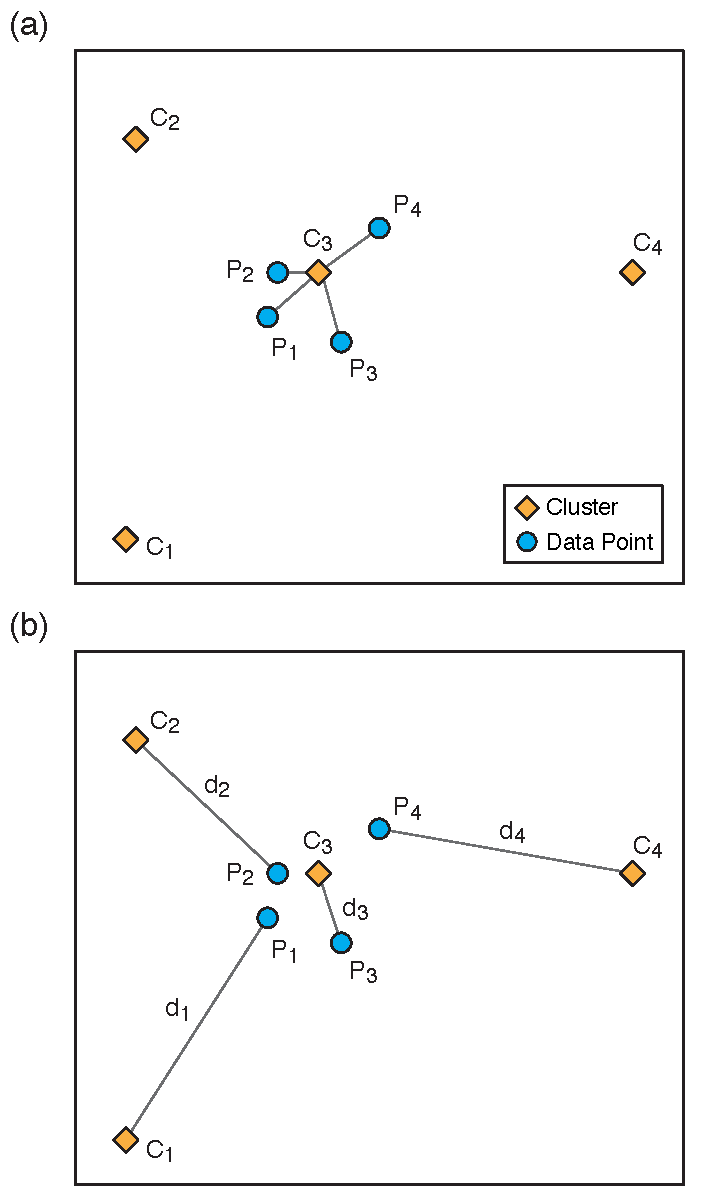
\includegraphics[width=\columnwidth]{figures/pdf/figure-04}
	\caption{Representation of the (a) ordinary, and (b) constrained \kmeans{} approaches for four data-points (P) and four cluster centers (C) in a 2D dataset space, where all the data-points are constrained to be cannot-link points. The color version of this figure is available only in the electronic edition.}
	\label{fig:k-means}
\end{figure}

This process is sensitive to the initial selection of the clusters and their centers. To mitigate this, constrained \kmeans{} introduces two types of constraints: must-link and cannot-link \citep{Wagstaff_2001_Proc}. The must-link constraint specifies instances in which two data-points must be linked, i.e., in the same cluster. The cannot-link constraint specifies instances in which data cannot be in the same cluster. This prevents the process from converging into a local minimum, and defines constrained \kmeans{} as a semi-supervised method. Figure \ref{fig:k-means} illustrates the differences between the standard and constrained \kmeans{} methods for a single clustering iteration on a small two-dimensional dataset.

In our implementation we limit the clustering to four validation categories: poor, fair, good, and excellent. The cluster centers are randomly selected at the start, but we apply constraints by adding 4 artificial stations with cannot-link conditions that are checked at the end of each iteration. These stations are associated with each type of cluster and have GOF scores equal to 3, 5, 7, and 9, across all metrics, thus they are representative of the validation categories. 

In the multi-dimensional space defined by the 11 GOF metrics used here, the distances are obtained using the Euclidean expression:
% 
\begin{equation}
	d(x_i, x_j) = \sqrt{ \sum_{l=1}^{n} \left( x_{i,l} - x_{j,l} \right)^2 } 
\end{equation}
% 
corresponding to the distance $d$ between the data-point $x_i$ and the cluster center $x_j$ in the $n$-dimensional domain, where $x_{i,l}$ is the $l$-th feature of the data-point $x_i$, and $x_{j,l}$ is the $l$-th feature of the cluster center $x_j$. It is, however, unpractical to expect the patterns defining the clusters to be observable across all features. Such high-dimensional issues are well known \citep[see, for instance,][]{Parsons_2004_ACM, Dy_2004_MLR}, and can be tackled using sub-spaces. Therefore, instead of analyzing all $2^{11}$ possible sub-spaces, we focus only on sub-spaces with 2, 3, and 4 dimensions, or features. In total, we analyze 550 sub-spaces, 55 sub-spaces with 2 features, 165 with 3, and 330 with 4.

Unfortunately, not all the sub-spaces will have clearly distinguishable clusters (i.e., some will not satisfy the cannot-link constraints even after a large number of iterations). Such sub-spaces are discarded, and all others are used to label the data. In an ideal case, each station will be labeled 550 times, and the final label is taken as the mode. For example, if after all the sub-spaces are accounted for, a station has labels $\left\{F, F, F, P, F, G, E, F, F\right\}$, where the labels $P$, $F$, $G$, and $E$ correspond to the poor, fair, good, and excellent category clusters, then such as station will be given a final label $F$. Once all the data is properly labeled, we proceed with the decision tree analysis.


% ===========================================================================================
%


% Although we do not expect to see the pattern that resulted from clustering using 11 features in presentation of only two, however, different studies show that the higher dimension reduce the effect of similarity based on distance. \citet{Parsons_2004_ACM} presented an illustrative example to show the effect of dimension in reducing the importance of the distance. Effect of higher dimensions in clustering has been well studied and many different methods are proposed to reduce this effect in the final results. Among them we can name  feature selection before, during, and after clustering, hybrid methods that use combination of methods to select the best subset of feature. \citet{Dy_2004_MLR} addressed two issues involved in developing an automated feature subset selection algorithm for unlabeled data. They illustrated the irrelevant and redundant features and proposed methods for evaluating candidate features using two performance criteria.

% Subspace analysis is another technique to address the challenges with higher dimensional data in clustering process. Subspace clustering is an extension of traditional clustering which looks for different pattern using subset of features.  \citet{Parsons_2004_ACM} provided a list of algorithm for conducting subspace clustering and also some potential applications for them. The most common factor among these algorithm is the process to find a group of best subspaces through optimization process. An n-dimensional dataset has $2^n$ subspaces where it could be very costly and time consuming to evaluate all of them.

% In this study we are interested in using those features who, in general, represent the simulation accuracy in 4 different categories. As a first step we use the constrained \kmeans{} clustering approach for all features, however, because of mentioned reasons the results are not easy to discuss or even evaluate. Although we have four groups of data, the question is which one should be considered as poor, fair, good, or excellent groups. Therefore, we apply a modified method of subspace clustering approach to cluster the stations. As we discussed earlier and presented in figures the constrained \kmeans{} method effectively put the stations in a cluster with considering the fact that our constrain stations should not be in the same cluster. High number of iteration leads the clustering process to follow the clustering concept that we are looking for which is clustering stations as poor, fair, good, and excellent. In our case number of possible subspace is $2^{11}$ where each features have two options wether belong to subspace or not. However, because of preserving the distance based criteria effects we limited the number of features in the subspace to be 2,3, and 4 features. Therefor we have 330,165, and 55 unique subspaces for 4D,3D, and 2D, respectively. We conduct a constrained \kmeans{} clustering analysis for each of these subspaces and repeat the algorithm. In some cases, it is not possible to distinguish all four cannot-link stations in different clusters. In this study we ignore these cases. We only use those combination of features that gives 4 unique clusters for the constraint points (hypothetical stations), therefore, we know for sure that all data within same cluster let's say with metric value 3, should be considered as poor. We also control the clusters to be consistent (we reformat numbers to assign cluster 1 to all group of stations that our first constraint belongs to them and so on). Finally, using 550 unique subspace clustering results, we assign the most frequent class to the station.





% and computes . These distances are then used as a criteria to determine the cluster to which cluster each data-point belongs. 

% ...


% \citet{Macqueen_1967_Proc} describes this method as a process for partitioning a $n$-dimensional population into $k$ sets on the basis of a sample. Its algorithm produces partitions that are reasonably efficient in the sense of within-class variance. It starts with a user defined number of clusters ($k$) and assigns a random mean value to each cluster (or randomly choose $k$ data-points and assigns them as cluster centers). After this, the algorithm computes the distances of all other data-points to the center of the cluster and uses the distance as a criteria to clustering the data points. Because the data resides in a multi-dimensional space (here defined by each metric), there are different ways of computing the distance of each data-point to the cluster's center. We use the Euclidean distance:
% % 
% \begin{equation}
% 	d(x_i, x_j) = \sqrt{ \sum_{k=1}^{n} \left( x_{i,k} - x_{j,k} \right)^2 } 
% 	\, ,
% \end{equation}
% % 
% where $n$ is the number of features and $d$ is the distance of $x_i$ and $x_j$ in $n$-$dimensional$ domain. 




% ===========================================================================================
%
% NEW TEXT PROVIDED BY NAEEM ON JAN 22
% Once the distance is computed, the algorithms labels the data based on the proximity of each point to each cluster, and computes the arithmetic mean value of the data for each cluster, and assigne that value as the updated location of each cluster's center. The algorithm repeats the steps unless the amount of updates among the cluster centers is less than a predefined tolerance value. The major problem with \kmeans{} algorithm is that it is sensitive to the selection of the initial partition and may converge to a local minimum of the criterion function value if the initial partition is not properly chosen. Another problem accompanying the use of \kmeans{} algorithm is the choice of the number of desired output clusters. \citep{Jain_1999_ACMCS}. Clustering is a subjective process. The same set of data items often needs to be partitioned differently for different application. In our application the number of clusters according to the literature is 4 (i.e., poor, fair, good, and excellent.) However, our initial attempts represents that the results are highly sensitive to the initial clusters' center. Therefore, we need to incorporate the experts knowlege in the process. 


% \citet{Wagstaff_2001_Proc}  demonstrated a modification of \kmeans{} clustering algorithm which uses the background information of the domain or dataset. The algorithm adds two types of constraints to the clustering including:
% 	% 
% 	\begin{itemize}
% 	\item{Must-link: constraints specify that two instances have to be in the same cluster.}
% 	\item{Cannot-link: constraints specify that two instance must not be placed in the same cluster.}
% 	\end{itemize} 
% 	% 
% The algorithm is described in detail in \citet{Wagstaff_2001_Proc}, however, in simple words, in the ordinary \kmeans{} process before assigning data to the closes cluster, it controls the must-link and cannot-link conditions. Therefore, in this case, the closest cluster's center is not necessarily the final cluster of the data.


% In a hypothetical assumption, if we have a pair of data and synthetic with GOF score of 3 for all metrics we could consider the overall simulation GOF as poor. This is also correct for 5,7, and 9 that we can assigne them fair, good, and excellent class, respectively. Therefore, we add 4 hypothetical stations into the dataset with GOF score of 3,5,7,and 9 for all metrics and we put them in cannot-link constraint. This assumption that originated from the experts knowledge, provides enough information to the algorithm to converge to the same final clusters and cluster centers after a reasonable amount of iteration. 

% Fig.~\ref{fig:con_kmeans} presents the difference between ordinary and constrained k-means clustering approach using 4 points and 4 cluster centers. Fig.~\ref{fig:con_kmeans}.a presents the \kmeans{} without constrained. According to the definition and the explanation in this section, the closest cluster center for each points will get the points. 	Fig.~\ref{fig:con_kmeans}.b represents the constrained \kmeans{} approach, where, the closest cluster center is not necessarily the final cluster. The data points can not be in the same cluster, in result,  we assign them to different clusters in this case to satisfy the Cannot-link criteria. The best configuration happens when we minimize the distance between cluster centers and points.

% ===========================================================================================
% 
% OLD STUFF DONE BY RICARDO FOR THE INTRO OF THIS SECTION
% 
% In machine learning, decision trees are classified as a supervised learning method, and the first step towards designing them requires that the data be labeled according to their attributes. The inherent attribute of our data are the GOF value themselves, but because of the multiplicity of metrics and the lack of clarity about how these relate to each other, we need to add labels to the data that are in accordance with the outcome attributes, i.e., in terms of the predefined validation quality levels. We label the data in our dataset by means of a clustering process. 

% There exist different methods for clustering data \citep[see Chapters 10 and 11 in][]{Han_2011_Book}, among which the \kmeans{} and constrained \kmeans{} clustering methods are the most widely used \citep{Jain_1999_ACMCS}. We note about these methods that the \kmeans{} approach is sensitive to the initial values chosen to be at the center of the clusters---especially in the case of data that are not clearly distinguishable---, whereas the constrained \kmeans{} method uses background knowledge to overcome this limitation. Because of its use of background information, the modified \kmeans{} method is considered as a semi-supervised process.





% ===========================================================================================
%
% SECOND ATTEMPT THAT WAS RECALLED BY NAEEM

% Once the distance is computed, the algorithms labels the data based on the proximity of each point to each cluster, computes the mean value of the data for each cluster, and updates the location of each cluster's center. \textcolor{red}{(How do we compute ``mean value'' and how do we recompute the ``center''? All what follows after this in the original text is too descriptive, and not specific enough. We need to go to the point and this is going in long description circles.)} 

% {\color{gray}
% 	The algorithm repeats the steps unless the amount of updates among the cluster centers is less than a tolerance value.  \kmeans{} clustering has been applied in different applications, however, there is no clustering technique that is universally applicable in uncovering the variety of structures present in multidimensional datasets. Therefore, clustering is a subjective process. The same set of data items often needs to be partitioned differently for different application. In result, it is essential for the user of a clustering algorithm to not only have a thorough understanding of the particular technique being utilized, but also to know the details of the data gathering process and to have some domain expertise; the more information the user has about the data at hand, the more likely the algorithm would be able to succeed in assessing its true class structure. Domain concept can play several roles in the clustering process, and a variety of choices are available to the practitioner \citep{Jain_1999_ACMCS}. 

% 	The major problem with \kmeans{} algorithm is that it is sensitive to the selection of the initial partition and may converge to a local minimum of the criterion function value if the initial partition is not properly chosen. Another problem accompanying the use of \kmeans{} algorithm is the choice of the number of desired output clusters. Several variant of the \kmeans{} algorithm have been reported in the literature. Some of them attempt to select a good initial partition so that the algorithm is more likely to find the global minimum value, another variation is to permit splitting and merging of the resulting clusters \citep{Jain_1999_ACMCS}. 

% 	In our application the number of clusters is not a problem and there is a consensus among researchers in the number of clusters (i.e., poor, fair, good, excellent), however, our initial attempts represent that the results are highly sensitive to the initial clusters' center. 

% 	Every clustering algorithm uses some type of knowledge either implicitly or explicitly. In this study the background knowledge is a series of hypothetical stations. We assume that there are four stations with score of 3, 5, 7, and 9 for all of their metrics. Based on the score limits in section.~\ref{validation_metrics} we know these stations belong to poor, fair, good, and excellent classes, respectively. These background knowledge could help the clustering processing to be in right direction regarding the fact that increasing dimension of data could increase noise in clustering and cause difficulty to better partitioning. \citet{Wagstaff_2001_Proc}  demonstrated a modification of \kmeans{} clustering algorithm which uses the background information of the domain or dataset. The algorithm adds two types of constraints to the clustering including:
% 	% 
% 	\begin{itemize}
% 	\item{Must-link: constraints specify that two instances have to be in the same cluster.}
% 	\item{Cannot-link: constraints specify that two instance must not be placed in the same cluster.}
% 	\end{itemize} 
% 	% 
% 	The algorithm is described in detail in \citet{Wagstaff_2001_Proc}, however, in simple words, in the ordinary \kmeans{} process before assigning data to the closes cluster, it controls the must-link and cannot-link conditions. Therefore, in this case, the closest cluster's center is not necessarily the final cluster of the data. Fig.~\ref{fig:con_kmeans} presents the difference between ordinary and constrained k-means clustering approach using 4 points and 4 cluster centers. Fig.~\ref{fig:con_kmeans}.a presents the \kmeans{} without constrained. According to the definition and the explanation in this section, the closest cluster center for each points will get the points.
	
% 	Fig.~\ref{fig:con_kmeans}.b represents the constrained \kmeans{} approach, where, the closest cluster center is not necessarily the final cluster. The data points can not be in the same cluster, in result,  we assign them to different clusters in this case to satisfy the Cannot-link criteria. The best configuration happens when we minimize the distance between cluster centers and points. Using this method at each step the algorithm redistribute the 4 hypothetical stations to satisfy the cannot-link constraint. The visual inspection of the figures also confirms the accuracy of the method. Doing this, in the next iteration this data manipulation leads the cluster center in a direction to have the hypothetical station in the cluster and loose those data that is in far other side direction of the hypothetical station. Therefore, the cluster tend to have all data that similar to the hypothetical station. \\
% 	The end product of the clustering process is groups of data. Analysis of these groups, individually, gives the idea about the clusters in terms of within class variation. In these analysis we mainly study the behavior of different features in each cluster and isolate only the most descriptive features to be used in the supervised classifier that assumes a given number of classes in the data set. In the next section we provide a basics of decision tree algorithm. 

% }

% In other words, the points cannot be in the same cluster. In the constrained \kmeans{} approach we redistribute the points such that the $\sum{d}$ becomes minimum.

% ===========================================================================================
%
% OLD NAEEM VERSION
% 
% Clustering is an unsupervised approach for grouping of data based on measure of similarity and it is considered as an exploratory activity as a part of data mining process \citep{Fayyad_1996_IEEE}. In each valid cluster, patterns are more similar in each other than they are to pattern belonging to a different cluster. Many clustering algorithms are developed for different application, however, study the difference of them is beyond the scope of this paper. In general, at the top level,  \citet{Jain_1999} distinguished the clustering approach into Hierarchical and Partitional approaches. Aside from differences in application and technical details in implementation, hierarchical methods produce nested series of partitions, while partitional methods produce only one. In this study we are interested in using partitional, distance based clustering algorithm, which is also known as \kmeans{} algorithm.  \citet{Macqueen_1967_Proc}  described a process for partitioning an $n$-$dimensional$ population into $k$ sets on the basis of a sample. The process appears to give partitions which are reasonably efficient in the sense of within-class variance. For numerical values, \kmeans{} algorithm starts with a user defined number of clusters (k) and assign a random mean value for each cluster (or randomly choose k data and assign them as cluster centers.) Then it computes the distance of data and cluster centers. A variety of distance measures are in use in different studies, however, we use the Euclidean distance through 

% \begin{equation}
% d(x_i,x_j)=\sqrt{\Sigma_{k=1}^{n}(x_{i,k} - x_{j,k})^2},
% \end{equation}

% where $n$ is the number of features and $d$ is the distance of $x_i$ and $x_j$ in $n$-$dimensional$ domain. After computing the distance of the points from each clusters' mean (center), the algorithm continues with labeling the data after the closest cluster. At the next iteration, it computes the mean value of data for each cluster and updates the clusters' centers. The algorithm repeats the steps unless the amount of updates among the cluster centers is less than a tolerance value.  \kmeans{} clustering has been applied in different applications, however, there is no clustering technique that is universally applicable in uncovering the variety of structures present in multidimensional datasets. Therefore, clustering is a subjective process. The same set of data items often needs to be partitioned differently for different application. In result, it is essential for the user of a clustering algorithm to not only have a thorough understanding of the particular technique being utilized, but also to know the details of the data gathering process and to have some domain expertise; the more information the user has about the data at hand, the more likely the algorithm would be able to succeed in assessing its true class structure. Domain concept can play several roles in the clustering process, and a variety of choices are available to the practitioner \citep{Jain_1999}. 

% The major problem with \kmeans{} algorithm is that it is sensitive to the selection of the initial partition and may converge to a local minimum of the criterion function value if the initial partition is not properly chosen. Another problem accompanying the use of \kmeans{} algorithm is the choice of the number of desired output clusters. Several variant of the \kmeans{} algorithm have been reported in the literature. Some of them attempt to select a good initial partition so that the algorithm is more likely to find the global minimum value, another variation is to permit splitting and merging of the resulting clusters \citep{Jain_1999}. 

% In our application the number of clusters is not a problem and there is a consensus among researchers in the number of clusters (i.e., poor, fair, good, excellent), however, our initial attempts represent that the results are highly sensitive to the initial clusters' center. 

% Every clustering algorithm uses some type of knowledge either implicitly or explicitly. In this study the background knowledge is a series of hypothetical stations. We assume that there are four stations with score of 3, 5, 7, and 9 for all of their metrics. Based on the score limits in section.~\ref{validation_metrics} we know these stations belong to poor, fair, good, and excellent classes, respectively. These background knowledge could help the clustering processing to be in right direction regarding the fact that increasing dimension of data could increase noise in clustering and cause difficulty to better partitioning. \citet{Wagstaff_2001_Proc}  demonstrated a modification of \kmeans{} clustering algorithm which uses the background information of the domain or dataset. The algorithm adds two types of constraints to the clustering including:\\
% \begin{itemize}
% \item{Must-link: constraints specify that two instances have to be in the same cluster.}
% \item{Cannot-link: constraints specify that two instance must not be placed in the same cluster.}
% \end{itemize} 
% The algorithm is described in detail in \citet{Wagstaff_2001_Proc}, however, in simple words, in the ordinary \kmeans{} process before assigning data to the closes cluster, it controls the must-link and cannot-link conditions. Therefore, in this case, the closest cluster's center is not necessarily the final cluster of the data. Fig.~\ref{fig:con_kmeans} presents the difference between ordinary and constrained k-means clustering approach using 4 points and 4 cluster centers. Fig.~\ref{fig:con_kmeans}.a presents the \kmeans{} without constrained. According to the definition and the explanation in this section, the closest cluster center for each points will get the points.
% Fig.~\ref{fig:con_kmeans}.b represents the constrained \kmeans{} approach, where, the closest cluster center is not necessarily the final cluster. The data points can not be in the same cluster, in result,  we assign them to different clusters in this case to satisfy the Cannot-link criteria. The best configuration happens when we minimize the distance between cluster centers and points. Using this method at each step the algorithm redistribute the 4 hypothetical stations to satisfy the cannot-link constraint. The visual inspection of the figures also confirms the accuracy of the method. Doing this, in the next iteration this data manipulation leads the cluster center in a direction to have the hypothetical station in the cluster and loose those data that is in far other side direction of the hypothetical station. Therefore, the cluster tend to have all data that similar to the hypothetical station. \\
% The end product of the clustering process is groups of data. Analysis of these groups, individually, gives the idea about the clusters in terms of within class variation. In these analysis we mainly study the behavior of different features in each cluster and isolate only the most descriptive features to be used in the supervised classifier that assumes a given number of classes in the data set. In the next section we provide a basics of decision tree algorithm. 


% \begin{figure}
%     \centering
%     \includegraphics
%       %  [width=\columnwidth]
%         [width=200px]
%         {figures/pdf/Figure_4.pdf}
%     \caption{ Representation of ordinary (a) and constrained (b) \kmeans{} approach. There are four data points (p) and four cluster centers (c) as a sample of $2$-$Dimensional$ dataset. All points are defined as cannot-link constraints. In other words, the points cannot be in the same cluster. In the constrained \kmeans{} approach we redistribute the points such that the $\sum{d}$ becomes minimum.}
%     \label{fig:con_kmeans}
% \end{figure}


% 
Decision tree learning is a method for approximating a target function, in which learned function is represented by decision tree \citep{Mitchell_1997_Book}. \citet{Quinlan_1986} demonstrated that the technology for building decision trees from examples is fairly robust. He summarized an approach to synthesizing decision trees that has been used in a variety of systems, and he describes one such system, ID3, in detail. Although ID3 algorithm is successful in most classification problems, it does not handle the numeric attributes and only one attribute at a time is tested for making decisions. \citet{Quinlan_1993} extended the ID3 algorithm and presented the C4.5 algorithm. Later on they added boosting capability to C4.5 and called it C5.0. The improved algorithm accepts both continues and discrete features and solves over fitting problem by pruning. Although there are many other algorithm for implementing decision tree, in this study we use the C5.0 algorithm. Discussing the algorithm in details is out of the scope of this paper. There are fairly good amount of references to study those details \citep[e.g.,][]{Mitchell_1997_Book,Quinlan_1993,Hornik_2009}.\\
In general, decision tree measures the effectiveness of an attribute in classifying the training data through information gain. According to  \citet{Mitchell_1997_Book}, information gain of an attribute is the expected reduction in entropy caused by partitioning the examples according to this attribute. If the target can take on $c$ different values the entropy is defined as
\begin{equation}
Entropy(S) = \sum_{i=1}^{c} -p_{i}\ log_2\ p_i,
\end{equation}

where $p_i$ is proportion of $S$ belonging to class $i$. Entropy measures the homogeneity of examples or dataset. Higher entropy means data is  fairly uniformly distributed among different classes. On the other hand lower entropy means data unequally distributed among classes. The extreme case happens when all data belong to one class which results in entropy equal to zero. Given entropy as a measure of impurity in a collection of training example the measure of the effectiveness of attribute is defined through information gain which is expected reduction in entropy caused by partitioning the examples according to this attribute. Gain of the attribute A is defined as 

\begin{equation}
Gain(S,A)\ =\ Entropy(S) - \sum_{v \in Values(A) } \frac{|S_v|}{|S|} Entropy(S_v)
\end{equation} 

where $Values(A)$ is the set of all possible values of attribute A, and $S_v$ is the subset of $S$ for which attribute $A$ has value $v$. Information gain is used by the algorithm in order to determine which is the better attribute for classifying the training example. The attribute with higher information gain will be the first option to separate the training data based on and grow to the lower nodes ( For more detailed examples refer to chapter 3 of \citet{Mitchell_1997_Book}). \\
We discussed the basic idea behind the decision tree algorithm, however, there are more details specially in dealing with outliers and noises which we address them through pruning approaches. In this study we use C5.0 package \citep{C50_2015} in R to conduct the decision tree algorithm. We discuss the input parameters in the section.\ref{classification_model}.  

% More text for use
%========================= \\
 %The method uses background knowledge to direct the clustering in an appropriate direction so the results are close to real data. Obviously there will be some features that is not obey the general pattern among these features. We will put aside those features. Then we try to modify those features to be able to use again in the processing. In the other words we will scale those features to obey the general trend. Anderson(2004) divided the stations into four main groups based on those stations scores. In hypothetical case were two signals are identical these scores should be 10. However, if they are not the same, but the scoring method provides similar results we should get a fairly close score for all matrics. In real cases the scores are different from one another. However, if we could define a metrics that gives a similar level of goodness of fit for all of them then we can for sure categorized the station in an appropriate group. In this study we define 4 hypothetical stations with score of 3,5,7, and 9 which represent middle points for poor, fair, good and excellent goodness of fit categories. Any station close to these stations should reflect the idea that they are at the same group. However, they are slightly different and we want to know why and how we can make them similar. So having these hypothetical stations and forcing the constrained k-means algorithm to put these stations in different groups we are able to bring the background knowledge into the process. So in the study we start with one attribute and cluster stations. According to figures (2D and 3D) we can argue that the background knowledge assisted the k-means clustering to cluster the stations, realistically. Meanwhile it could not force the clusters to have a cluster centers as those points.  We assign the most frequent stations' cluster to that station. Then we study the score variation in each group and see if they have a uniform behavior if not we can further study the potential problems with that score and probable scaling factors to make it obey the pattern. We also analyze the effect of velocity model, earthquake, orientation, frequency band in the final results. 
%Based on having class for each station in the study we develop a decisition tree to provide the group of simulation for Los Angles Basin earthquakes.  \\

%To do list: \\

%Another approach to go is considering all data without separating for earthquake, velocity model, and so on. Then try to put them in one cluster. Those stations which are in the cluster but are in extreme case, remove from the data base. \\
%Analyze inside each cluster, provide normal distribution, if data looks ok keep it, if not remove those features. \\
%Normally majority of dimensions are irrelevant in high dimensional data. These irrelevant dimensions can hide clusters in noisy data and confuse the clustering algorithm. \\
%Try different method and cluster data, then find the points that clustered currently then use that points as a must link condition. \\
%We can not show data with 10 attributes in graph, however, we can generate a set of statistical figures of changing these values in the figure.\\ 
%If using a feature cause to not able to fit the station in any class we remove it or give a factor to put in the right class.\\
%in the end we want to have all stations as constrained. In other word, we start from 1D and if there is a station that is always in the same group we added it in constraint points. then we move to the 2D and we continue the same until we have all station as constraint.\\
%Constraint helps the clustering to get the same results after good amount of iterations.\\
%========================= \\